% timetags
%
\documentclass[10pt,dvips]{article}
%\documentclass[10pt,twocolumn,dvips]{article}
\usepackage{epsfig}
\usepackage[english]{babel}
%\usepackage{fancyheadings}
%\usepackage[T1]{fontenc}
%\usepackage[latin1]{inputenc}
%\usepackage{twocolumn}
%\usepackage{verbatim,moreverb,doublespace}
%\usepackage{rotate,lscape,dcolumn,array,rotating,latexsym}
%
%\input{epsf}
%
% for somebody (I forget now !)
%\textwidth 175mm
%\textheight 225mm
%\topmargin -4.5mm
%
% for somebody else (I also forget now !)
%\textwidth 6.6in 
%\textheight 239mm
%\topmargin -15mm
%\leftmargin -2.0in
%
% for HPCA (IEEE single-column format)
\textwidth 6.875in
\textheight 8.875in
\topmargin -0.6in
\oddsidemargin 0mm
\evensidemargin 0mm
%
%
% some publishers want no page numbers for final print
%\pagestyle{empty}
%
\begin{document}
%
%
\title{Preserving Program Dependencies in a Distributed Microarchitecture}
%
%
\author{
D. Morano\\
Northeastern University\\
dmorano@ece.neu.edu
}
%
%
% some publishers do not want a data in the final print
\date{}
%
\maketitle
%
% uncomment the following for page with no page numbers (for IEEE)
%\thispagestyle{empty}
%
%
\begin{abstract}
We discuss how {\em time tags} can be used for the enforcement of
program dependencies.
Time tags can serve as the basic ordering enforcement mechanism
when large numbers of instructions are executing concurrently.
Proposed and future microarchitectures can have hundreds or several hundreds
of instructions in flight simultaneously and using standard 
reservation
tags, physical register addresses, and reorder buffers do not scale
well for very large instruction windows.
The design, use and management of time tags will
be discussed.  
We also provide simulation data for an example microarchitecture
that takes advantage of time tags for its dependency ordering.
\end{abstract}
%
%
\section{Introduction}
%
In this paper we discuss a means by which time tags can be used
to enforce proper program dependencies while allowing
massive out-of-order execution by a suitable (and likely large)
microarchitecture.
Several studies into instruction level parallelism
have shown that there is parallelism within
typical programs that is not yet exploited by existing
microarchitectures ~\cite{Gon97,Lam92,Uht95}.  
Suitable microarchitectures for extracting this ILP would need to
execute a very large number of instructions in parallel.
However tracking and enforcing the dependencies for these
large microarchitectures presents significant implementation
difficulties.  The use of time tags appears to be mechanism well suited
for this task.

We are proposing to use time tags to maintain 
and enforce correct program order for all flow dependencies whether
they be registers, memory values, or instruction control-flow predicates.
It may be noted that the \textit{time} aspect of time tags
refers to program-order time and not real time.
The goal is to allow for massive speculative out-of-order 
instruction execution
in real time while providing a means of tracking program order
time.

Section 2 will provide some high level applications for and background on
the use of time tags.  Specifically, microarchitectural capabilities
that are likely desirable in future machines, and which may be implemented 
more easily using time tags, are presented.
Section 3 presents a description of time tags and how they would
fit into a potential microarchitecture.  
Also discussed are
some optional microarchitectural features
that can be facilitated once time tags are used as
a program dependency enforcement mechanism.
Section 4 briefly presents a proposed microarchitecture
that uses time tags for all of its dependency tracking and enforcement.
Simulated results from this microarchitecture are also presented.
We summarize in Section 5.
%
%
\section{Application and Background}
%
Current microarchitectures generally employ mechanisms such as a
Register Update Unit or Reorder Buffer(s) ~\cite{Bannon95,Smith95,Kessler98}
to enforce
proper program dependencies for registers and predicates.
Memory dependencies are often enforced through the use of
snooping the memory store queue or some other memory disambiguating
mechanism ~\cite{Sohi96}.
The use of time tags to coordinate and enforce correct program
order can reduce or eliminate both routing congestion and
contention for conventional machine structures such as
register scoreboards \cite{Thornton64} 
or the architected register file associated
with the use of reservation stations~\cite{Anderson67}.

In those microarchitectures
that perform speculative execution, there is also
the need to access the reorder buffer.  This becomes very problematic
as the number of instructions being speculatively executed concurrently
grows~\cite{Palacharla97}.  
Whether speculative instruction operand
results are stored in data registers within the reorder buffer or if the
results are stored in extra physical registers that hold both architected
and temporary values, the contention for the centralized resource is
the same.
Further, future microarchitectures may employ value speculation
~\cite{lipasti96exceeding,lipasti97performance,gonzalez98limits}
as well as control-flow speculation.
Time tags would appear to be a good candidate for unifying, to some
extent, the tracking of value dependencies along with control-flow
dependence.

Several microarchitectures have also been proposed that perform multipath
execution.  Some of these are described by Wang ~\cite{Wang90}, 
Uht and Sindagi ~\cite{Uht95},
Heil and Smith ~\cite{Heil96},
the PolyPath by Klauser et al ~\cite{Klauser98},
and a simultaneous multithreading oriented approach by
Wallace et al \cite{Wallace98}. 
In order to accommodate multipath execution, we 
employ a \textit{path ID} similar to that described by Skadron
and Ahuja ~\cite{Skadron01}.

Some newly proposed microarchitectures are also addressing
the desire to execute control-independent instructions
beyond the join of conditional branches.
Some of these are described by 
Sankaranarayana and Skadron ~\cite{Sank01a,Sank01b}, Cher and
Vijaykumar ~\cite{Cher01}, and Uht et al ~\cite{Uht01}.
In our present work, we also desire to provide for the speculative
execution and reuse of control-flow independent instructions
after conditional branches.  We will use time tags
to facilitate the ordering of operands and instruction execution in this
sort of circumstance also.

The Warp Engine~\cite{Cleary95} used time tags.  
However their implementation
was somewhat cumbersome ; utilizing 
floating point numbers and machine-wide parameter
updating.  
We will employ a simpler representation of program-order time for our time
tags.
%
%
\section{Time Tags}
%
A time tag is a small
integer that uniquely identifies the position of an instruction
or an operand in program ordered time.
Both instructions and operands are tagged with these values.
Typically, time tags take on small positive values to
indicate the position of an instruction in program ordered
time with respect to the most recently committed and retired
instruction, which can be thought of having a time tag value
of minus one.
The oldest dispatched instruction in flight that is neither 
yet committed nor
squashed would usually have the time tag value of zero.
Those instructions in flight, and therefor being
in future program
ordered time, take on increasingly larger values the further ahead
they are in the program ordered instruction stream.
Likewise, certain operands that are created by instructions 
(the outputs of that instruction) would take on
the same time value as its instruction.  
This thus provides
the fundamental means by which proper operand dependency order can
be tracked and enforced.
As instructions, or groups of instructions,
having the lowest valued time tags
are retired, all of the time tags for all instructions and
operands are decremented by the number of instructions just
retired.  This will keep the next instruction in program-ordered
time, the next instruction to be retired in order,
having the time tag value of zero.
Other variations for the assignment and management of the
values are also possible (and have been used) but thinking 
of the oldest dispatched
and not yet retired instruction as having the value zero is
most illustrative for this presentation.

In the arrangement described so far, negative valued time tags may still
be used depending on the particulars of the microarchitecture
that they might be employed for.  In such cases, instructions
themselves would never take on negative values since there
is no need to retain them after they are finally retired.
However, operands might still take on negative valued time tags and this
would indicate that they have already been committed but that
their program-order relationship to each other is desired
to be maintained for some purpose.
An example might be when memory operands are committed but
still need to be snooped in a store queue of some sort.
Rather then forcing a FIFO storage arrangement for those committed
memory values, it may be more expedient to use time tags
for the same purpose.
%
%
\subsection{Operands}
%
Operands for instructions can be of varying types and
different microarchitectures may want to treat each type
somewhat differently.
At least three types of instruction operands may be identified
for most microarchitectures.
These are register, memory, and predicate operands.
Some microarchitectures may want to allow for more speculative
flexibility of certain operands while not allowing
as much speculation for other types.

For most microarchitectures, registers are the primary instruction
operand and will thus, rightly, deserve the most attention.
These register operands would consist of both those
that are input to the instruction as well as those that
are outputs from the instruction.
Typically, all machines with register oriented instruction set
architectures (ISAs) could
likely benefit from having register operands time tagged.

However, it may be quite advantageous to additionally tag 
memory and possibly predicate operands as well.
The time tagging of memory operands allows them to be
treated as flexibly and as speculatively as register operands
might be.  
Memory operands only apply to those instructions that
perform memory load/store type functions.  
A load-type instruction
can be thought of having one or more input memory operands
and a store-type instruction likewise has one or more output
memory operands.  With this understanding, load/store instructions
can now be handled in ways very similar to all register-only
oriented instructions.

For predicate operands, two types need to be distinguished.
One type is a part of the ISA of the machine and
is therefor visible to programmers.
A predicate operand of this type would be
used in an ISA such as the iA-64, for example.
For our purposes, this sort of explicit predicate operand
is identical to a register operand (discussed above) and
is simply treated as such.
Not as clear is the use of predicate operands
that are not a part of the ISA and are therefor not visible
to the programmer.
This type of predicate in entirely maintained by the microarchitecture
itself but still essentially forms an additional input operand
for each instruction.
This single bit operand is what is used to
predicate the instruction's committed execution, the same as
if it was explicit in the ISA.
This input predicate thus enables or disables its associated
instruction from producing its own new output operand.
It should be noted that, at any time, any instruction can
always still be allowed to execute but that only the output results
of that instruction execution must be made available or not depending
on the instruction's input predicate operand.
For microarchitectures that support these microarchitecture-only
predicate operands, they too can be time tagged, thus allowing
them the same degree of out-of-order flexibility similar
to register or memory operands.
Finally, note that even ISAs that sport predicate registers
can also independently employ predication of instructions within the
microarchitecture.
%
%
\subsection{Multipath Execution}
%
Not all microarchitectures may uses multiple speculative
execution paths but we plan for that case anyway.
Some extra complications may arise for those microarchitectures
that allow for multiple simultaneous speculative execution paths.
There are several ways in which multiple
execution paths can be tracked but some care needs to be
applied in the context of also using time tags.
Generally, a new speculative path may be formed
after the encounter of each additional conditional branch
in the instructions stream.  Execution is not speculative
for those instructions just following the last committed
instruction but all instructions are speculative after
the first unresolved conditional branch is encountered.
At least two options are available for assigning time tags
to the first instruction following each output of a conditional
branch.  

One option is to dynamically follow
each output path and assign successively higher time tag values
to succeeding instructions.
Another option is to try to determine if the \textit{taken} outcome
of the branch joins with the \textit{not-taken} output instruction
stream.  If a join is determined, the instruction following
the \textit{not-taken} output path can be assigned a time value
one higher than the branch itself, while the first instruction
on the \textit{taken} path would be assigned whatever value
it would have gotten counting up from the first instruction
on the \textit{not-taken} path.
Further, both options may be employed simultaneously in the
same microarchitecture.

In both cases, there will exist instructions in flight
that both have the same value for their time tag.  
Likewise,
operands resulting from these instructions would also share
the same time-tag value.
For our purposes, this ambiguity is resolved through the
additional of a \textit{path-ID} value.
This path ID would also be tagged to all instructions and
operands just as the time tags are.
With the addition of the path-ID, in addition to time tags,
a fully unique address space is now possible for
all instructions that may be in flight.
%
\subsection{Names and Renaming}
%
We are now in a position to define a name space that
uniquely specifies all instructions and operands that
may be in flight at any time.
For instructions, names for them can be uniquely created
with the concatenation of the following components :
%
\vspace{-0.05in}
\begin{itemize}
\vspace{-0.1in}
\item{a path ID}
\vspace{-0.1in}
\item{the time tag assigned to a dispatched instruction}
\vspace{-0.1in}
\end{itemize}   
%
For all operands, unique names would consist of :
%
\vspace{-0.05in}
\begin{itemize}
\vspace{-0.1in}
\item{type of operand}
\vspace{-0.1in}
\item{a path ID}
\vspace{-0.1in}
\item{time tag}
\vspace{-0.1in}
\item{identifying address}
\vspace{-0.1in}
\end{itemize}   
%

Generally, the type of the operand would be \textit{register},
\textit{memory}, or \textit{predicate}.
Remember that ISA visible predicate are treated just as regular
data registers within the microarchitecture itself.
The use of this component for operand names may not be
necessary depending on how the different operand types
are transfered among instructions.
This is discussed more later.
Again, the path ID and time tag are as discussed previously.
The identifying address of the operand would differ
depending on the type of the operand.
For register operands, the identifying address would be
the name of the architected register.
All ISA architected registers are typically provided a
unique numerical address.  These would include the
general purpose registers, any status or other non-general
purpose registers, and any possible ISA predicate registers.
For memory operands, the identifying address is just the
programmer visible architected memory address of the corresponding
memory value.
Finally, for predicate operands, the identifying address
may be absent entirely, for some microarchitectures, or
might be some address that is used within the microarchitecture
to further identify the particular predicate register in question.
We have explored microarchitecture predication schemes that 
have used both options above.

Now that all instructions and operands can have
unique names within the microarchitecture of a machine,
additional options open up for new microarchitectures
that were not as obvious or exploitable in previous
machines.
For example, if each instruction in an issue slot
retains a copy of its input or output operands (whatever
they may be), effectively a full renaming of
all operands will have occurred for all instructions
in flight in the machine.  
All false dependencies are now automatically avoided.
There would be no need to limit instruction dispatch or to limit speculative
instruction execution due to a limit on the number of non-architected
registers available for holding temporary results.
Since every possible operand has a unique name and is available
to be read in some way, both all needed ordering information
and the associated necessary operand values to match
a particular ordering would be available.
This feature can be used powerfully
to eliminate the need for physical register renaming,
register update units, or reorder buffers.
The sum of the issue slots in the machine would effectively serve
as a sort of reorder buffer in themselves.
We will next
explore how operands are transferred from
instruction to instruction while enforcing the necessary
true program dependencies for proper execution.
%
%
\subsection{Operand Forwarding and Snooping}
%
As with microarchitectures not using time tags,
operands resulting from the execution of instructions
are broadcast forward for use by waiting instructions.
As expected, when operands are forwarded, they are done so
by transferring not only the identifying address of the operand
and its value but also the time tag and a potential path-ID (for
those microarchitectures using multipath execution).
This tag will be used by subsequent 
instructions 
(later in program order time)
already dispatched
to determine if
the operand should be {\em snarfed}~\footnote{snarfing entails snooping
address/data buses, and when the desired address value is detected, 
the associated data value is read} 
as an input that will trigger
the execution of its loaded instruction.

The information associated with each operand that is
broadcast from one instruction to subsequent ones
is referred
to as a {\em transaction}, and generally consists of :
%
\vspace{-0.05in}
\begin{itemize}
\vspace{-0.1in}
\item{transaction type}
\vspace{-0.1in}
\item{operand type}
\vspace{-0.1in}
\item{path ID}
\vspace{-0.1in}
\item{time tag of the originating instruction}
\vspace{-0.1in}
\item{identifying address}
\vspace{-0.1in}
\item{data value for this operand}
\vspace{-0.1in}
\end{itemize}   
%
This above information is typical of all operand transactions.
True flow dependencies are enforced through the continuous snooping of
these transactions by each dispatched instruction residing in an issue
slot that receives the transaction.
Each instruction
will snoop all operands that are broadcast to it but
an operand forwarding interconnect fabric may be devised so that
transactions are only sent to those instructions that primarily
lie in future program-ordered time from the originating instruction.  
More information on operand forwarding interconnection networks
is presented in a later section.
More details on transactions for register, memory, and
predicate forward operations are also presented later.

Figure \ref{fig:source} shows the registers inside an 
issue slot used for the snooping and snarfing of 
one of its input operands.  
The 
{\em time-tag},
{\em address}, and
{\em value} registers are reloaded with new values on each snarf,
while the
{\em path} and
{\em instr. time-tag} are only loaded when an instruction is
dispatched to the active station.
The operand shown is typical for source registers, a source memory
operand, or an instruction execution predicate register.
%
\begin{figure}
\centering
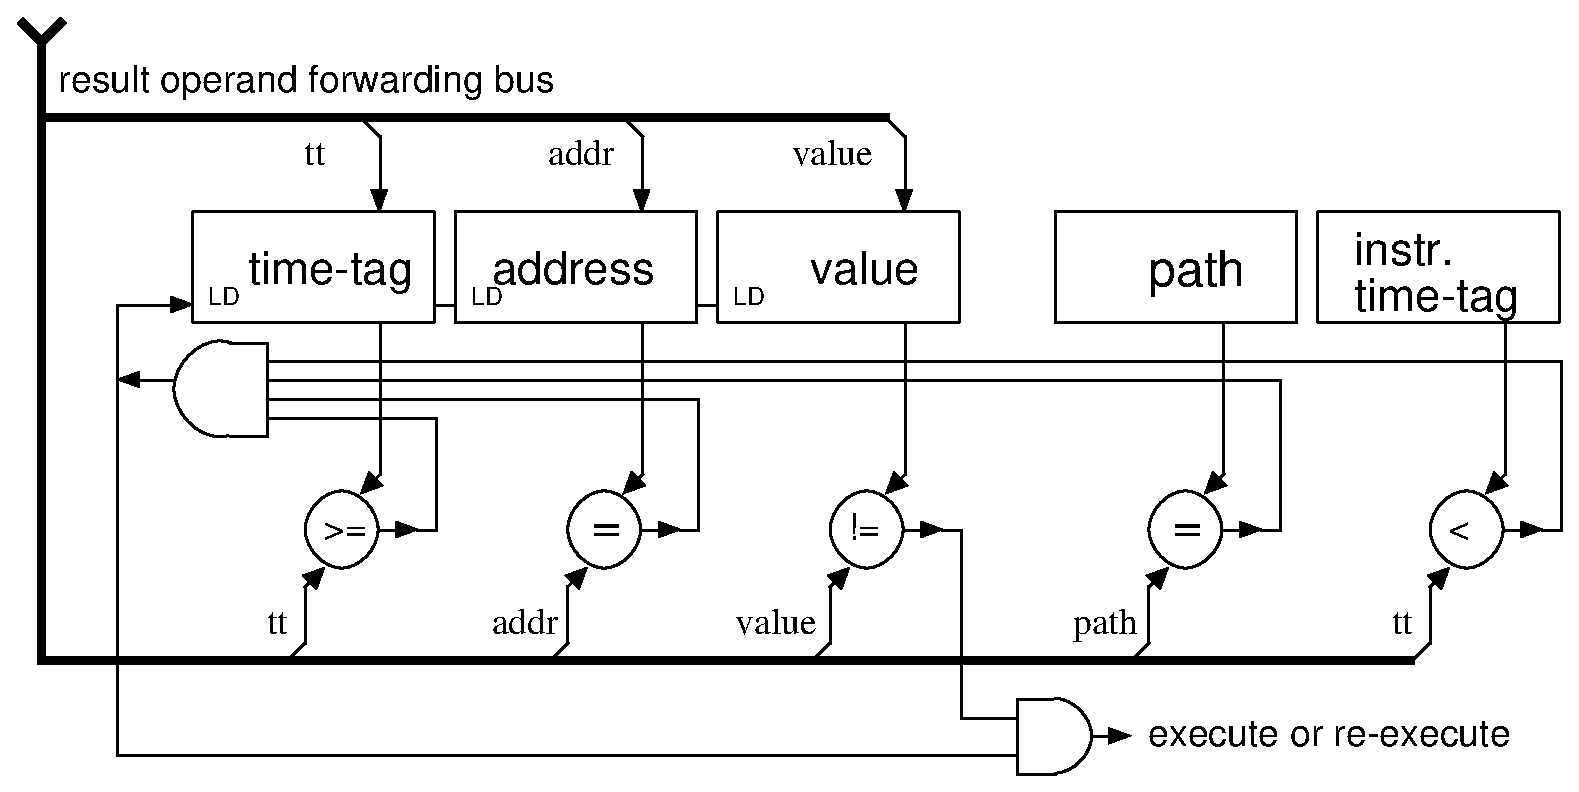
\epsfig{file=source.eps,width=5.0in}
\caption{{\em Instruction Source Operand.} The registers and snooping
operation of one of several possible source operands is shown.
Just one operand forwarding bus is shown being snooped but
typically several operand forwarding buses are snooped simultaneously.}
\label{fig:source}
\end{figure}
%

If the
path ID and the identifying address of the operand matches any of
its current input operands, the instruction then checks
if the time tag value is less than its own assigned time tag,
and greater than or equal to the time tag value of the last
operand that it snarfed, if any.  
If the snooped data value is
different than the input operand data value that the active
station already has, a re-execution of the instruction is initiated.
This simple rule will allow for the dynamic discovery of
all program dependencies during instruction execution while 
also allowing for maximum concurrency to occur.
%
%
\subsection{Result Forwarding Buses and Operand Filtering}
%
The basic requirement of the interconnection fabric is that it must be able
to transport operand results from any instruction to those
instructions with higher valued time tags.  This corresponds
to the forwarding of operands into future program ordered time.
There are several choices for a suitable interconnection fabric between
instruction issues slots.
A simple interconnection fabric could consist of one or more
buses that simply interconnect all issue slots.
Although appropriate for smaller sized microarchitectures,
this arrangement does not scale as well as some other alternatives.
A more appropriate interconnection fabric that would allow
for the physical scaling of the microarchitecture may be one in which
forwarding buses are segmented with active repeaters between
the stages.
This arrangement exploits the fact that, for example, register lifetimes
are limited ~\cite{Franklin92,Sohi95}.
Registers being forwarded to instructions lying close
in future program-ordered time will get their operands quickly
while those instructions lying beyond the repeater units
will incur additional delays.
In addition to allowing for physical scaling, it also offers
the opportunity for filtering out some operands that do
not need to be forwarded beyond a certain point.
Another possibility for the operand forwarding fabric is
to have separate buses for each type of operand.
This sort of arrangement could be used to tailor the available
bandwidth provided for each type of operand.  It could also
allow for a different interconnection network to be used
for each type of operand also.  We have explored several of
these possible variations already.

The opportunity to provide active repeaters between forwarding bus
segments also opens up a range of new microarchitectural
ideas not easily accomplished without the use of time tagging.
Different types of active repeaters can be optionally used.
Further, different types of repeaters can be used for
the different types of operands.
Some can just provide a store-and-forward function while
another variation could also store recently forwarded operands
and filter out (not forward) newly snooped operands that
have already been forwarded previously. 
The latter type of forwarding repeater unit is termed a
\textit{filter unit}.
This feature can be used to reduce the operand traffic
on the forwarding fabric and thus reduce implementation costs.
For example, for memory operands, a cache (call it a \textit{L0 cache})
can be situated inside a \textit{memory filter unit} (MFU)
and can hold recently requested memory operands.
This can reduce the demand on the L1 data cache and the rest
of the memory hierarchy by satisfying some percent of memory
operand loads from these caches alone.
Register filter units (RFUs) are also possible and can reduce
register transfer traffic similarly to the MFUs.
%
%
\subsection{Operand Forwarding Strategies and Bus Transactions}
%
Although we have so far described the operand forwarding mechanism
in simple terms as being the broadcasting of it 
to those ASes with higher valued 
time tags, there are some additional details that need to be
addressed for a correctly working forwarding solution.
These details also differ depending on whether operands for
register, memory, or predicates need to be forwarded.
There are many possible strategies for forwarding of operands
(and of operands of differing types). 
We now briefly outline three such strategies.
One of these is suitable for registers.
Another is suitable for registers or memory operands.
The third is oriented for the forwarding of predicates.
These three strategies are termed \textit{relay forwarding},
\textit{nullify forwarding}, and \textit{predicate forwarding}
respectively.
In general, each forwarding strategy employs bus transactions
of one or more types to implement its complete forwarding solution.
The particulars of these transactions are described for each
of the forwarding strategies.
%
%
\subsubsection{Relay Forwarding}
%
This forwarding strategy is quite simple but is also entirely
adequate for the forwarding of register operands.
In this strategy, when a new register operand needs to be forwarded
from an active station, the standard operand information, as 
previously described
in a general, is packaged up into what is termed
a \textit{register store} transaction.
This transaction type consists of :
%
\vspace{-0.05in}
\begin{itemize}
\vspace{-0.1in}
\item{a transaction ID of \textit{register store}}
\vspace{-0.1in}
\item{the path ID on which this instruction is executing}
\vspace{-0.1in}
\item{the time tag of the originating active station}
\vspace{-0.1in}
\item{the register address}
\vspace{-0.1in}
\item{the value of the register}
\vspace{-0.1in}
\end{itemize}   
%
A request is made to arbitrate for an outgoing forwarding bus
and this transaction is placed on the bus when it becomes available.

When the instruction associated with an active station gets
a new input operand, it will re-execute producing a new
output operand.  In this forwarding strategy, the new output
operand is both stored locally within the active station itself
and is sent out on the outgoing forwarding buses
to subsequent (higher time-tag valued) active stations.
Previous values of the instruction's output operand is also
snooped as if it was an input operand and is also stored locally
within the active station.
It should also be noted that if the enabling execution predicate
for the current instruction changes, either from being enabled
to disabled or visa versa, a new output operand is forwarded.
If the instruction predicate changes from disabled to enabled,
the output operand that was computed by the instruction os
forwarded.  If the instruction predicate changes from enabled
to disabled, the previous value of the output operand (before being
changed due to the instruction execution) is forwarded.
That previous value is available to the active station because
it gets snooped as if it was an additional input.
Newly forwarded operands will always superseded and previously
forwarded operands.
With this strategy, instructions that are located in the program
ordered future will eventually always get the correct
value that will end up being the committed value if the
current instruction ends up being committed itself (ends
up being predicated to execute).
This is an elegant forwarding strategy and
the simplest of the forwarding strategies investigated so far, and
is a reasonable choice for the handling register operands.
The inclusion of the time tag in the transaction is the
key element that allows for the correct ordering of
dependencies in the committed program.
%
\subsubsection{Nullify Forwarding}
%
There are limitations to the applicability of the previously
discussed forwarding strategy (relay forwarding).
That strategy depends upon the fact that the address of the
architected operand does not change during the life time of
the instruction while it is in an active stations.
For example, the architected addresses for register operands
do not change for instructions.  If the instruction takes
as an input operand a register \textit{r6} for example,
the address of the operand never changes for this particular
instruction (it stays \textit{6}).
This property is not generally true of memory operands.
The difficulty with memory operands is that many memory
related instructions determine the address of a memory operand
value from an input register operand of the same instruction.
Since we allow for instructions to execute and re-execute
on entirely speculative operand values, the values of
input register operands can be of essentially any value
(including a wilding incorrect value) and thus the
address of a memory operand can also change during the during
that the instruction is in flight within the active station.
This presents a problem for the correct enforcement of
memory operands, and dependencies among them, in the entire program.
If we examine the case of a memory store instruction,
when it
re-executes acquiring a new memory store value, the address of that
memory store may also have changed !  
We cannot simply forward that new memory operand (address and value)
as with the relay forwarding strategy above.  The reason is
that we would not be superseding the previous memory operand
that we forwarded previously that quite likely had a different
architected address.  Rather, we need some way to cancel the effect of
any previously forwarded memory operands.
This present forwarding strategy does just that.

In this strategy, memory operands that need to be forwarded
employ a similar transaction as above for registers (described
in the context of relay forwarding) but would instead have
a transaction ID of \textit{memory store} and would
include the memory operand address and its value (along with the
path and time-tag information).
However, when an instruction either re-executes or
its enabling predicate changes to being disabled, a different
type of forwarding transaction is sent out.
This new type of transaction is termed a \textit{nullify transaction}
and has the property of nullifying the effect of a previous
store transaction to the same architected operand address.
This transaction type consists of :
%
\vspace{-0.05in}
\begin{itemize}
\vspace{-0.1in}
\item{a transaction ID of \textit{memory nullify}}
\vspace{-0.1in}
\item{the path ID on which this instruction is executing}
\vspace{-0.1in}
\item{the time tag of the originating active station}
\vspace{-0.1in}
\item{the memory operand address}
\vspace{-0.1in}
\item{the value of the memory operand}
\vspace{-0.1in}
\end{itemize}   
%
When this transaction is snooped by subsequent ASes,
for those ASes that have a memory operand as an input
(that would be for instructions that load memory values in
one way or another)
a search is made for a match of an existing memory
operand as usual but if a match is detected,
the time-tag of that particular memory operand is set to
a state such that any future \textit{memory store} transaction,
regardless of its time-tag value, will be accepted.
Further, on reception of this \textit{memory nullify} transaction,
a request is sent backwards in program order for a memory
operand with the desired memory address.
The transaction that represents a request for a memory
operand would consist of :
%
\vspace{-0.05in}
\begin{itemize}
\vspace{-0.1in}
\item{a transaction ID of \textit{memory request}}
\vspace{-0.1in}
\item{the path ID on which this instruction is executing}
\vspace{-0.1in}
\item{the time tag of the originating active station}
\vspace{-0.1in}
\item{the memory operand address}
\vspace{-0.1in}
\end{itemize}   
%
Of course, the memory address for the operand desired
needs to be in the transaction but it is not as obvious why
the originating AS's time tag is also included.  In some
interconnection fabrics, the time tag is included in backwarding
requests to limit the scope of the travel of the transaction
through the execution window.  This same scope-limiting function
is usually performed for forward going transactions as well.
When the request is sent backwards in program order, previous
ASes or the memory unit itself will eventually snoop
the request and respond with another \textit{memory store}
transaction.
As discussed, this forwarding strategy is very useful for memory
operands but it can also be used for register operands with
appropriate changes to the applicable transaction elements.
Again, the inclusion of a time tag value is what allows
for proper operand dependencies (whatever they may be for
any particular forwarding strategy) in the committed program.
%
\subsubsection{Predicate Forwarding}
%
There are several ways in which instructions can be predicated
in the microarchitecture.  
These predication mechanisms are not discussed in
this paper but two such mechanisms are can be found in
documents by Uht et al ~\cite{Uht01} and Morano ~\cite{Morano02}.
For microarchitectures that predicate all program instructions
within the microarchitecture itself (not visible at the ISA
level of abstraction), predicate register values are essentially
operands that need to be computed, evaluated, and forwarded
much like register or memory operands.
Each instruction computes its own enabling predicate by
snooping for and snarfing predicate operands that are forwarded
to it from previous instructions from the program-ordered past.
Depending on the particular predication mechanism used,
relay forwarding (described above) may be a suitable (if not good) choice 
for handling the forwarding of predicate operands.
However, some predication mechanisms need additional transaction
types (besides a base store transaction) to communicate.
The predication mechanism described by Morano ~\cite{Morano02}
requires three transaction to fully implement.
That mechanism was employed for the data presented in a later section
and the transactions for that mechanism
are briefly described here.

This predication strategy requires two store-type transactions
rather than just one.  These two transactions are similar
to other operand store transactions (like for register or memory
operands)
but one of these holds two values rather than just one.
The first of these is the \textit{region predicate store}
transaction and consists of :
%
\vspace{-0.05in}
\begin{itemize}
\vspace{-0.1in}
\item{a transaction ID of \textit{region predicate store}}
\vspace{-0.1in}
\item{the path ID on which this instruction is executing}
\vspace{-0.1in}
\item{the time tag of the originating active station}
\vspace{-0.1in}
\item{the region predicate value}
\vspace{-0.1in}
\end{itemize}   
%
This transaction is very analogous to a register or memory
store but instead is used to forward a single bit value (the
current \textit{region predicate} for instructions following the
AS that forwarded the transaction).  A region predicate
is a single bit that determines the execution status
(enabled or disabled) for instruction that lie beyond the
not-taken output path of a conditional branch.
This particular transaction could be forwarded by either
a conditional branch or by a an instruction that was not
a control-flow-change instruction.  In the
case of a non-control-flow-change instruction, the only
predicate value that makes sense is the same as its
own enabling predicate and so only one value need
be forwarded.

In the case of a conditional branch instruction,
there are two possible output predicates that can be in
view.  One is for the not-taken output path from the branch.
The other is for the taken output path.
In order to forward both values for those instructions
in program-ordered future, the other store transaction
type (mentioned previously) us used.
This transaction consists of :
%
\vspace{-0.05in}
\begin{itemize}
\vspace{-0.1in}
\item{a transaction ID of \textit{branch target predicate store}}
\vspace{-0.1in}
\item{the path ID on which this instruction is executing}
\vspace{-0.1in}
\item{the time tag of the originating active station}
\vspace{-0.1in}
\item{the branch target instruction address}
\vspace{-0.1in}
\item{the region predicate value}
\vspace{-0.1in}
\item{the branch target predicate value}
\vspace{-0.1in}
\end{itemize}   
%
This is identical to the previous \textit{region predicate store}
transaction but also includes the instruction address
for the target of the conditional branch (the \textit{taken} address)
and the single bit predicate
governing the execution status for instructions
following the target of the conditional branch in program-ordered
future.

Finally, for the predication mechanism employed in the present
work, a third transaction is used to invalidate a previously
forwarded branch target predicate.  This transaction is
a \textit{branch target invalidation} and consists of :
%
\vspace{-0.05in}
\begin{itemize}
\vspace{-0.1in}
\item{a transaction ID of \textit{branch target invalidation}}
\vspace{-0.1in}
\item{the path ID on which this instruction is executing}
\vspace{-0.1in}
\item{the time tag of the originating active station}
\vspace{-0.1in}
\item{the branch target instruction address}
\vspace{-0.1in}
\item{the time tag of the branch target predicate to be invalidated}
\vspace{-0.1in}
\end{itemize}   
%
This is similar to other such invalidation transactions in
that when it is snooped by ASes in the program-ordered future,
a search is made for some state (in this case some predicate
register state) that matches the given transaction criteria.
The inclusion of the second time tag in this transaction allows
for certain efficiencies that are particular to the predication
mechanism described.

For predicate forwarding, as we have seen for register and
memory forwarding, time tags play the vital role in
identifying and preserving the ordering of all operands.
In many ways, all operands (whether they be registers, memory,
or execution predicates) require the use of time tags to
determine the relative ordering of events in a microarchitecture
that otherwise lets all instructions execute and re-execute
wildly out of order in real time with respect to each other.
%
%
\subsection{Execution Example}
%
A simple execution example using time tags 
is shown in Figure \ref{fig:example1}.
%
\begin{figure}
\centering
\begin{tabular}{|l|l|l|l|l|l|}
\hline 
TT&instr&t1&t2&t3&t4\\
\hline 
0&r3 := 1&&&~~~~&\\
&&r3=1&&&\\
\hline 
1&r4 := r3 + 1&&r3=1&&~~~~\\
&&&r4=2&&\\
\hline 
2&r3 := 2&&&&~~~~\\
&&&&r3=2&\\
\hline 
3&r5 := r3 + 2&&r3=1&&r3=2\\
&&&r5=3&&r5=4\\
\hline 
\end{tabular}
\caption{{\em Example Instruction Execution.} The time tags for sequential
program instructions are on the left.  Real time is show advancing
along the top.  For each real time interval, input operands are shown
above any output operands.}
\label{fig:example1}
\end{figure}
%
In this example we show how register operands are created and
snarfed in real time.
Four instructions are listed along with the time tag (TT) assigned to them
on the left.  Real time progresses to the right and time four periods
are identified.  In time period \textit{t1}, the instruction with 
TT=0 executes and creates its output operand \textit{r3}.
This operand is forwarded to succeeding instruction in program
ordered future time.  In time period \textit{t2}, instructions
at TT=1 and TT=3 have snarfed this operand since it was one of
their inputs and met the snarfing criteria.  
These two instructions execute in parallel and
create their output operands.  Of course, the output for
instruction at TT=3 is incorrect but that can not be determined
at this point in real time.  In time period \textit{t3},
instruction at TT=2 executes creating its output operand.
That operand gets forwarded and is snarfed by the instruction at
TT=3 because it met the snarfing criteria.  That instruction
re-executes as a result in time period \textit{t4} thus
creating its correct output.  All instructions are now ready
for commitment with their correct outputs.
%
%
\section{A Proposed Microarchitecture Using Time Tags}
%
In this section we present a proposed microarchitecture
that uses time tags as its basic dependency enforcing mechanism.
The microarchitecture is ISA independent (can be applied to
any ISA) and offer most of the features that are likely desirable
in future machines.  Among these are control-flow speculation
and execution along with execution reuse of control-independent
instructions beyond the joins of conditional branches,
prediction of both register and memory values, and multipath execution.
Further, the proposed microarchitecture has a structure that allows
for its size (numbers of various units) to scale without adverse
implementation feasibility or significant performance loss.
%
%
\subsection{Hardware Description and Operation}
%
The most significant feature of this microarchitecture is
that it makes use of an instruction issue slot that retains
its decided instruction until it is ready to be retired 
(either committed or squashed) from execution.
This is similar to what Lipasti and Shen employed in a microarchitecture
proposed by them ~\cite{Lip97}.
Our use of the issue slot is also similar to the old idea
of reservation stations ~\cite{Tom67} since they are positioned
in silicon in close proximity to execution resources.  However,
unlike reservation stations and more like an issue window,
several of our instruction issue slots can share the same
execution resources.
We call our adaptation of the issue slot an 
{\em Active Station} (AS) where the idea of \textit{active}
illustrates that instructions dispatched to them will
re-execute as necessary until retired.  

Our Active Stations are laid out in silicon 
in a two dimensional grid whereby sequentially
dispatched instructions (in program order) are assigned to 
sequential ASes down a column of
the two dimensional grid of ASes.  
Time tags are thus assigned to the ASes in the same order
that instructions were dispatched to them.
As expected, these time tags have values starting at zero
and
incrementing up to one minus the total number of
ASes in the machine.

Associated with each group of ASes are execution resources.
We term each such resource
a \textit{Processing Element} (PE).  
A group of active stations along with their execution resource
is termed a \textit{Sharing Group} (SG).
We also term the two dimensional
grid of ASes, along with their interspersed execution units (PEs),
the {\em Execution Window}.
This arrangement is shown in Figure \ref{fig:window}.  
There are four SGs shown, each with six ASes and one PE.
The total height of each column consists of six ASes and there
are two columns of SGs and four columns of ASes.
%
\begin{figure}
\centering
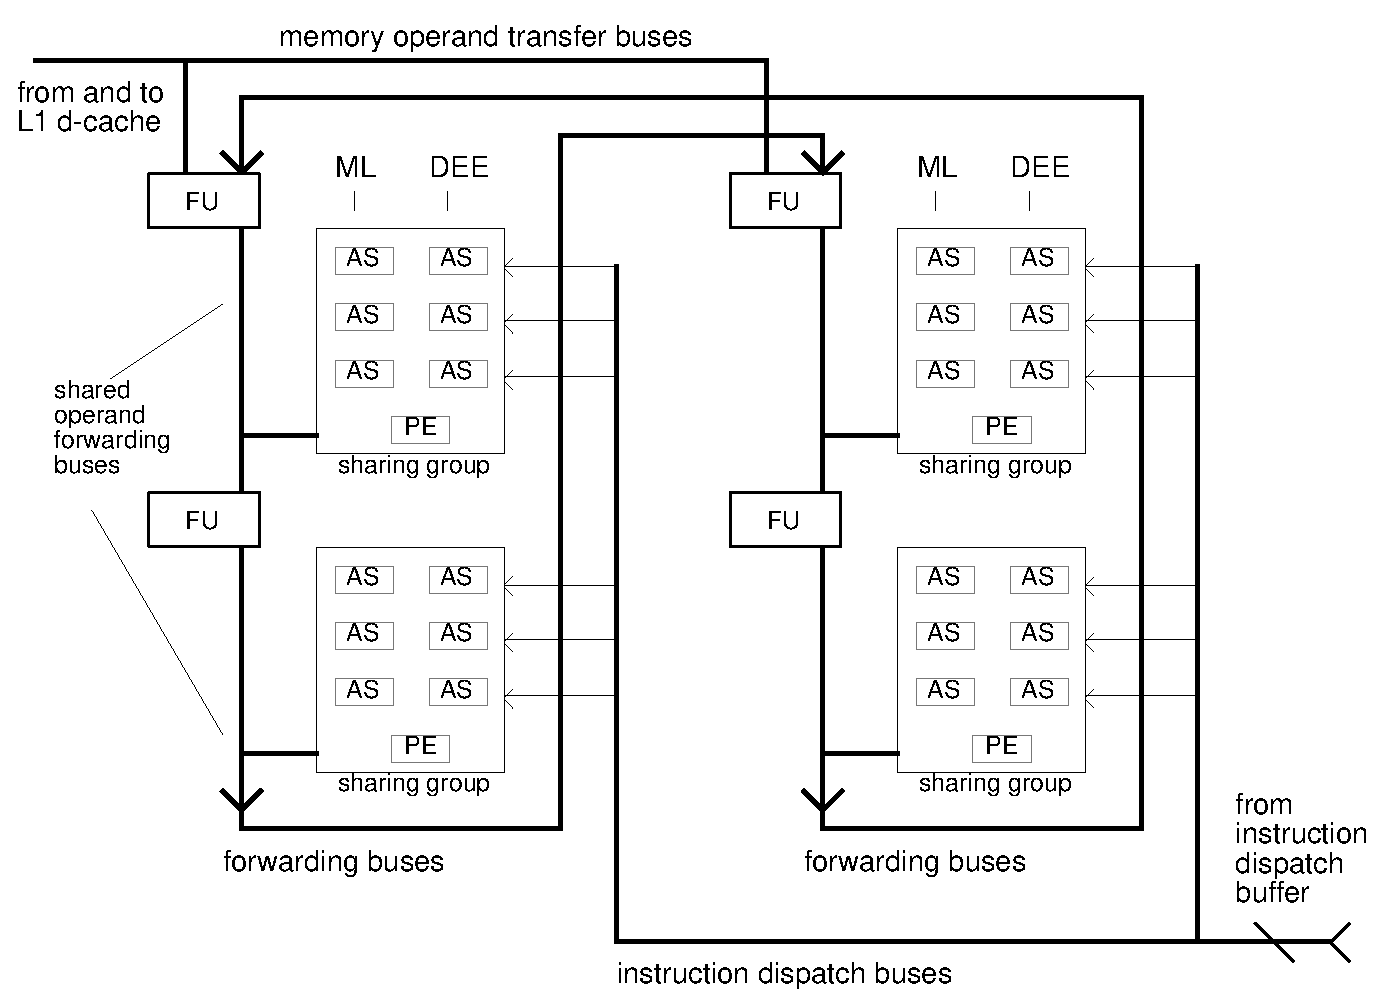
\epsfig{file=window.eps,width=5.0in}
\caption{{\em Execution Window.} Shown are four sharing groups
each with six active stations and one shared processing element.
There are six rows of ASes in each column of the entire arrangement.}
\label{fig:window}
\end{figure}
%
In this microarchitecture, instructions are dispatched to an entire
column of ASes simultaneously.
At a maximum, new instructions can be dispatched to a column every
cycle.  
Logically, the columns form a ring with the lower valued
time tags on the left and the higher valued time tags on
the right.  
As a column of instructions retires, that column 
receives
newly dispatched instructions that take on time tag values
that will become the highest values in the machine.
However all time tags are decremented
when a new set of instructions is dispatched to a column.
Thus the logical renaming of columns (and their constituent ASes)
is effected.
In addition to the ASes receiving time tags for tracking program
order, all operands in the microarchitecture are also tagged
with time tags.  The usually comparisons (discussed previously)
of time tags and operands architected addresses provides
the basic dependency enforcing mechanism.
Instructions generally re-execute when they snarf new
input operands but they are also allowed to use value prediction
for input operands not yet acquired through snooping.

This microarchitecture also takes advantage of the fact that
instructions are dispatched to the ASes in program order down
each column and continuing at the top of the next column to its right.
Due to this physical ordering of the ASes, operand results
only need to be forwarded to those ASes that lie below it, in its
own column, and to those ASes in columns logically to the
right.  
This arrangement provides for the opportunity to have 
a scalable interconnect
fabric connecting the SGs to each other since
there is no real need to provide connectivity
from any single AS to prior ASes in the machine.
The interconnection fabric for this microarchitecture
is also segmented and both RFUs and MFUs are employed.
Although not shown in Figure \ref{fig:window},
three separate sets of forwarding buses were used for
each of the three types of operands (register, memory,
and predicate).
%
%
\section{Simulation Results and Discussion}
%
Using an execution-driven simulator, we ran
SpecInt-2000 and SpecInt-95 programs on our
time-tagged microarchitecture.  
Our goal here was to evaluate
the instruction per clock (IPC) that was possible using
the microarchitecture.
Ten benchmark programs were used
in all.  
Seven programs are from the SpecInt-2000 suite and
three are from the SpecInt-95 suite.  
These programs were
chosen in order to get a variety of execution behaviors.
The microarchitecture simulated supports 
the MIPS-1 ISA (big endian), with some MIPS-2
instructions also supported in order to accommodate code residing in
the SGI system libraries which use them.
All programs were compiled using the vendor SGI compiler on
the SGI IRIX 6.4 operating system.
Programs were compiled with
standard optimization ({\tt -O}) for primarily the MIPS-1 ISA ({\tt -mips1}).
The first 600 million instructions of all programs were
executed.  Data were only gathered after the execution of
the first 100 million instructions (a total of 500 million).
The default features of the machine simulated are
given in Table \ref{tab:params}.
%
\begin{table}
\begin{center}
\caption{{\em General machine characteristics.}
These machine parameters are used for all simulations as
the default except where one of these parameters may be varied.}
\label{tab:params}
\begin{tabular}{|l|l|}
\hline 
L0 cache size&32 words\\
\hline 
L1 I/D cache access latency&1 clock\\
\hline
L1 I/D cache size&64 KBytes\\
\hline
L1 I/D block size&32 bytes\\
\hline
L1 I/D organization&2-way set associative\\
\hline
L2 cache access latency&10 clocks\\
\hline
L2 cache size&2 MBytes\\
\hline
L2 block size&32 bytes\\
\hline
L2 organization&direct mapped\\
\hline
main memory access latency&100 clocks\\
\hline
forwarding unit minimum latency (all)&1 clock\\
\hline
forwarding-bus latency (all)&1 clock\\
\hline
number of register forwarding buses&2\\
\hline
number of predicate forwarding buses&2\\
\hline
number of memory buses&1\\
\hline
branch predictor&PAg\\
\cline{2-2}
 & 1024 PBHT entries\\
\cline{2-2}
 & 4096 GPHT entries\\
\cline{2-2}
 & saturating 2-bit counter\\
\hline
\end{tabular}
\end{center}
\end{table}
%
The data in Table \ref{tab:ipc1} contains IPC 
results for a range of machine sizes.
All machines simulated also contained two forwarding buses for
register operands, two forwarding buses for predicates, and
one forwarding bus for memory operands.
All forwarding buses incur a bus transfer delay of 1 clock.
Further, each forwarding unit encountered (different for different
machine sizes) has a minimum latency of 1 clock.
All simulated machines, regardless of size, have forwarding buses
that span eight sharing groups.  This illustrates how the bus
length can be constant with respect to the machine size thus allowing
for physical scalability of the machine.
Machine sizes are basically characterized by
Each of the machine configurations in Table \ref{tab:ipc1} consists of three
numbers that give the rows of sharing groups, the number
of AS rows per sharing group, and the total number of 
columns respectively.  The number of sharing group rows times the
number of ASs per sharing group is the total number of
AS rows in a configuration.  The product of all three
numbers gives the total number of ASes in the machine and therefor
the number of instructions that may be in flight 
simultaneously
(having
possibly speculatively executed already).
%
\begin{table}
\begin{center}
\caption{{\em Benchmark IPC results for various machine sizes.}
Different machine sizes are characterized by their
geometries consisting of the three-number entries along the
top of the table: SG rows per column, AS rows per SG, and
SG columns.}
\label{tab:ipc1}
\begin{tabular}{|l|c|c|c|c|c|c|c|c|}
\hline 
config&
8-4-8&8-4-12&12-4-8&8-8-8&8-12-8&8-16-8&16-8-8&32-8-8\\
\hline
\hline 
bzip2&4.1&4.1&4.3&4.9&5.2&5.5&4.9&5.1\\
\hline 
compress&4.1&4.3&4.3&4.7&4.8&4.8&4.8&4.9\\
\hline 
crafty&3.7&3.8&3.8&4.1&4.2&4.1&4.1&4.4\\
\hline 
gcc&3.1&3.1&3.1&3.3&3.3&3.3&3.4&3.6\\
\hline 
go&4.1&4.6&4.7&5.1&5.5&5.4&5.3&6.0\\
\hline 
gzip&4.8&5.0&5.2&6.1&6.5&6.4&6.4&6.5\\
\hline 
ijpeg&6.2&7.2&7.8&9.5&12.3&13.1&12.0&12.3\\
\hline 
mcf&3.5&3.5&3.6&4.3&4.7&5.3&4.5&5.0\\
\hline 
parser&3.5&3.7&3.5&3.9&4.0&3.9&3.9&4.4\\
\hline 
vortex&4.2&4.4&4.7&4.8&4.9&4.6&4.9&5.1\\
\hline 
\hline 
H-MEAN&3.8&4.2&4.3&4.7&4.9&5.06&4.9&5.2\\
\hline
\end{tabular}
\end{center}
\end{table}
%
Generally, as the number of ASs increases,
the resulting IPCs also increase, but there are diminishing returns.
A significant IPC gain is achieved, for example, when increasing the
size of the machine from the 8-4-8 geometry (256 ASes) to the 8-8-8 geometry
(512 ASs).  This is an increase in IPC of approximately 17.8\% on the
harmonic mean across all benchmarks.  However, doubling the number
of ASs again (the number of instructions in flight
in the e-window simultaneously) to 1024 with the 16-8-8 machine geometry,
the harmonic mean IPC only increases by about 3.4\%.  Even an
alternative geometry (the 8-16-8 geometry) also having 1024 ASs
gives a harmonic mean IPC of 4.96, an increase of approximately 5.6\%
over the 8-8-8 geometry.
Comparing the 8-16-8 geometry with the 16-8-8 geometry (both having
1024 ASes), the results from each are fairly similar with the
8-16-8 geometry edging out the 16-8-8 when all benchmarks are
considered.  However, for some benchmarks (like GCC and VORTEX)
the IPC are lower with the 8-16-8 geometry.  This suggests that
there is little benefit in just increasing the number of AS
rows per sharing group after some point (16 in the present) case
since contention for the single common processing logic starts
to limit performance.
With the current state of this microarchitecture research,
the best tradeoff of resources and IPC results would appear
to be with the machine geometry of 8-8-8.  This consists of 512
ASs and the associated bus interconnects between them. 
Without the use of time tags as an operand dependency enforcing
mechanism, it is not clear how this arrangement could otherwise be 
implemented
in current or near-term process technologies due to interconnection
and contention problems that would arise.

A better look at the potential of this microarchitecture is
presented by the IPC data in Table \ref{tab:ipc2}.
Some of the configurations presented previously, 
in Table \ref{tab:ipc1},
are repeated but this time they were executed with a relaxed
assumption about the branch prediction accuracy guiding the
fetching and dispatching of instructions into the e-window.
In this data set, 100\% branch prediction accuracy was
assumed in an attempt to see what might be possible with this
general microarchitectural approach as research continues to
make possible i-fetch improvements.
%
\begin{table}
\begin{center}
\caption{{\em Benchmark IPC results for various machine sizes
when assuming 100\% branch prediction accuracy guiding i-fetch.}
Different machine sizes are characterized by their
geometries consisting of the three-number entries along the
top of the table: SG rows per column, AS rows per SG, and
SG columns.}
\label{tab:ipc2}
\begin{tabular}{|l|c|c|c|c|}
\hline 
config&
8-4-8&8-8-8&16-8-8&32-8-8\\
\hline
\hline 
bzip2&9.0&12.4&15.5&16.3\\
\hline 
compress&8.1&12.2&16.2&17.6\\
\hline 
crafty&6.1&9.3&14.7&21.7\\
\hline 
gcc&7.1&12.3&17.3&21.2\\
\hline 
go&9.0&12.3&17.3&21.2\\
\hline 
gzip&7.6&10.0&11.2&11.5\\
\hline 
ijpeg&9.2&14.4&18.7&20.2\\
\hline 
mcf&6.1&8.2&10.1&12.0\\
\hline 
parser&7.3&10.9&14.6&17.0\\
\hline 
vortex&6.4&10.1&15.2&21.7\\
\hline 
\hline 
H-MEAN&7.3&10.8&13.3&16.9\\
\hline
\end{tabular}
\end{center}
\end{table}
%
In this IPC data, results continue to improve up through the
32-8-8 machine geometry.
Any realization of a machine with this number of speculative
instructions in flight (2048 in this case) is clearly not
feasible given current operand enforcement methods like
a reorder buffer.  Contention for access to it would be too great
given current and foreseeable silicon limitations.
%
%
\section{Summary}
%
We have presented a method for tracking and enforcing
program dependencies through the use of time tags.
Register, memory, and predicate dependencies can all be
managed with time tags.
We have also described several microarchitectural
features are either enabled or become more feasible through
the use of time tags for dependency enforcement.
We have also presented a proposed microarchitecture that
used time tags throughout and which allows for
control-flow speculation and
reuse of
control-flow independent instructions,
data speculation,  and multipath execution.
The proposed microarchitecture is also physically scalable
through the use of a segmented operand forwarding fabric.
The use of time tags allows for a degree of out-of-order
execution that is not easily enforceable using any other
mechanism due to either routing congestion or access contention
problems.
We also presented results that indicates that this general 
approach appears to be quite
promising as compared with the existing more conventional program
dependency enforcement mechanisms.
Some work on much larger machine configurations has already
suggested that achieving IPC numbers in the 10s on general integer
sequentially-oriented program codes is possible.
%
\bibliographystyle{latex8}
\bibliography{timetags}
%
\end{document}
%
%
%
%
